\section{Methods}

In order to demonstrate that the DISHTINY platform selects for detectable hierarchical transitions in individuality, we performed experiments where cell-like organisms evolved parameters for manually designed strategies controlling relevant aspects of behavior including resource-sharing, reproductive decision-making, and apoptosis.
We will first cover the design of the DISHTINY platform then move on to describe the simple cell-like organisms we used to evaluate the platform.

\subsection{DISHTINY}

\begin{figure*}[t]
\begin{center}
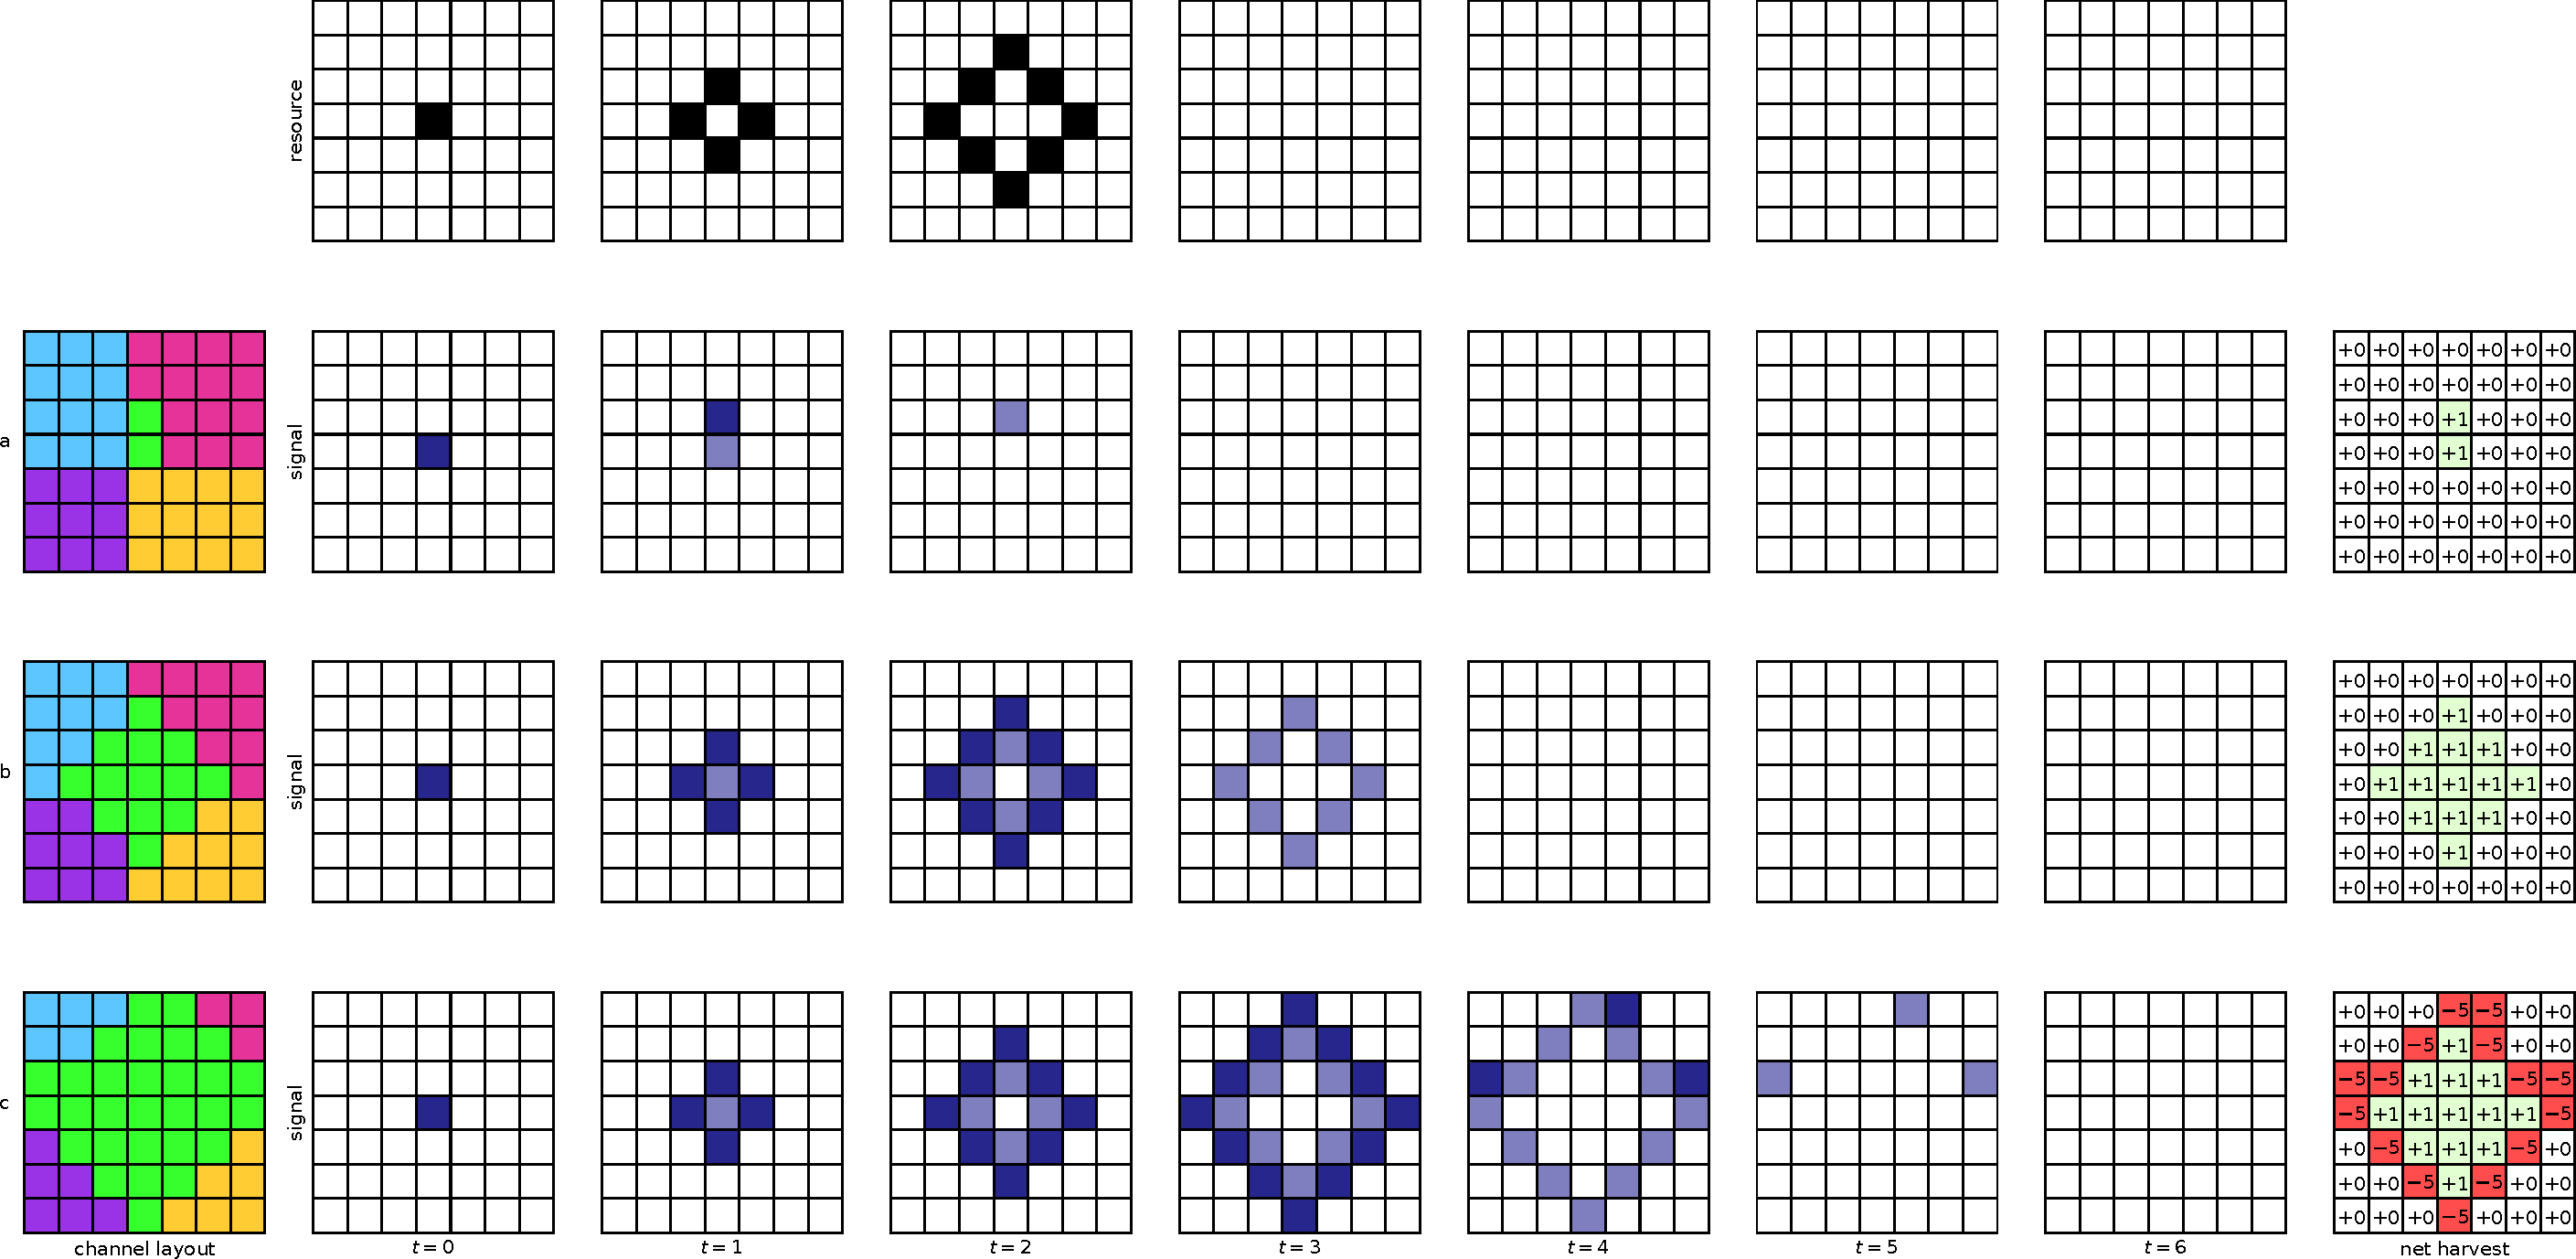
\includegraphics[width=2.0\columnwidth]{img/explanatory}
\caption{Activation-quiescence signaling, and net resource collection for three different channel configurations during a single resource wave events.}
\label{fig:explanatory}
\end{center}
\end{figure*}


DISHTINY centers around cell-like organisms, which represent the atomic level of individuality, distributed over a toroidal grid.
Over discrete timesteps called ``updates,'' the cell-like organisms collect a single continuous-valued resource.
Once sufficient resource has been accrued, cell-level organisms may pay a cost of $-8.0$ resource to place a daughter cell on an adjoining tile of the toroidal grid (i.e. reproduce).
Any cell-level organism existing on that adjoining tile is destroyed and replaced with the daughter cell.

As shown at the top of Figure \ref{fig:explanatory}, resources appear in diamond-shaped waves that emanate from a single point.
With each simulation update, the resource wave advances one grid tile outward, disappearing when it reaches a predefined limit.
In order to collect resource as it passes overhead, cell-level organisms must enter an activated state from their resting ready state.
The cell-like organism at the starting position of a resource wave is automatically set to the activated state from the ready state.
At the next update, this activated cell-like organism automatically induces neighboring cell-like organisms registered to the same signaling channel to enter the activated state and itself transitions to a temporary quiescent state.
Subsequently, the newly activated cell-like organisms activate ready neighbors registered to the same signaling channel and themselves enter a temporary quiescent state.
In this manner, cells sharing the same signaling channel activate coincident with the expanding resource wave.
As shown Figure \ref{fig:explanatory}$b$, the rate of resource collection for a cell-level organism is determined by the size and shape of of its same-channel signaling network;
small or fragmented same-channel signaling networks will frequently miss out on resource as it passes overhead.

Each cell-like organism pays a resource cost when it enters the activated state.
This cost is outweighed by the resource collected such that cell-like organisms which activate in concert with a resource wave derive a net benefit.
Recall, though, that resource waves have a limited extent.
Cells that activate outside the extent of a resource wave or activate out of sync with the resource wave (due to an indirect path from the cell that originated the signal) pay the activation cost but collect no resource.
Cells that frequently activate erroneously use up their resource and die.
In our implementation, organisms that accrue a resource debt of $-11$ or greater are killed.
This scenario is depicted in Figure \ref{fig:explanatory}$c$.

In this manner, ``Goldilocks'' --- not to small and not too big --- same-channel signaling networks are selected for.
In our implementation, resource waves are seeded at a single location drawn  with uniform probability from the toroidal grid.
Based on this location, resource wave seeds are tiled over the toroidal grid such that their limits touch but do not overlap.
All waves start and are updated synchronously;
when they complete, the next batch of resource waves is seeded.
This process ensures that selection for ``Goldilocks'' same-channel signaling networks is uniformly distributed over the toroidal grid.

Cell-level organisms may control the size and shape of their same-channel signaling group by strategic control of reproduction.
Three choices are afforded: whether to reproduce at all, where among the four adjoining tiles of the toroidal grid to place their offspring, and whether the offspring should be registered to the parent's signaling channel or should instead be registered to a random channel ID (int the range 1 to $2^{22}$).
No guarantees are made about the uniqueness of a newly-generated channel ID, but chance collisions are rare.

Hierarchical levels are introduced into the system through multiple instantiations of this resource wave/channel-signaling scheme.
In our experiments, we worked with two resource wave/channel-signaling levels, identified here as level zero and level one.
On level zero, resource waves extended a radius of four toroidal tiles.
On level one they extended a radius of twelve toroidal tiles.
On both levels, activated organisms netted $+1$ resource from a resource wave, but suffered an activation penalty of $-5$ if no resource was available.
Due to the different radii of resource waves on different levels, level zero selects for smaller same-channel signaling networks and level one selects for larger same-channel signaling networks.

We enforced hierarchical nesting of these same-channel signaling networks during reproduction:
daughter cells may inherit neither channel ID, just the level one channel ID, or both channel IDs.
Daughter cells may not inherit only the level zero channel while having a different level one channel.
The distribution of IDs across the level one and level zero channels can be envisioned by analogy to political countries and territories.
Each country (i.e. level-one channel network) may have one or many territories (i.e. level-zero channel network).
However, no territory spans more than one country.
Figure \ref{fig:outcome_grids} depicts hierarchically nested channel states at the end of three evolutionary runs.

Channel IDs enable straightforward detection of an evolutionary transition in individuality.
Because common channel IDs may only arise systematically through inheritance, common channel IDs indicate a close hereditary relationship in addition to a close cooperative relationship.
Because new channel IDs arise first in a single cell, same-channel signaling networks are reproductively bottlenecked, ensuring meaningful reproductive lineages at the level of the same-channel signaling network.
To recognize an evolutionary transition in individuality, we therefore evaluate
\begin{enumerate}
\item Do cell-level organisms with the same channel ID choose to share resources (e.g. cooperate)?
\item Is there division of reproductive labor between members of the same channel (e.g., do cell-level organisms at the interior of a network cede reproduction to those at the periphery?)
\end{enumerate}
If these conditions are met among cell-level organisms sharing the same level zero channel, we can conclude that a zeroth-level transition in individuality has occurred.
Likewise, if these conditions are met among cell-level organisms sharing the same level one channel, we can conclude that a first-level transition in individuality has occurred.

\subsection{Organisms}

We performed our experiments using cell-level organisms comprised of a set of 15 floating-point parameters, each controlling a specific lifestyle strategy component.
These cell-level organisms are in no way inherent to the DISHTINY platform, but were merely developed to study the platform.
On reproduction, mutation was applied to each parameter independently with probability $0.00005$.

The altruism parameters ($A_0$ and $A_1$) control the probability that an organism declines to replace an adjoining organism that shares the same level-zero ($A_0$) or level-one ($A_1$) channel ID with their offspring.
Mutation is performed by a redraw from the uniform distribution $U(-0.5,1.5)$ clamped to the range $[0,1]$.

Resource allocation is controlled by the $P_{c}$, $P_0$, and $P_1$ parameters.
The $P_{c}$ parameter controls the proportion of resource collected into and paid from a cell's individual resource stockpile, while the $P_0$ and $P_1$ parameters, respectively, control the proportion of resources going into and out of resource pools shared by organisms with identical level zero and level one channel IDs.
These parameters are initialized by a draw from $U(0.0, 1.0)$ and mutated by addition of a normal value drawn from $N(0.0,0.2)$ with the result clamped to the range $[0,1]$.
The set $P_{c}, P_0, P_1$ is always normalized to sum to 1.

Channel resource pools are identical to an organism's individual stockpile, except that any deficit is distributed evenly among the individual organism's stockpile.
On every update, cell-level organisms can spend from their individual stockpile to reproduce or from a channel pool, with priority given to cell-level organisms nearest to the centroid of that pool's members.
As such, pool-funded reproduction fills in a same-channel signaling network from the inside out and can result in diamond-shaped same-channel signaling networks.
(Distance is measured using the taxicab metric.)

Channel caps $C_0$ and $C_1$ limit the size of same-channel signaling networks.
When an organism reproduces, it checks the size of its level zero signaling network against $C_0$ and the size of its level one signaling group against $C_1$.
If neither cap is met or exceeded, then the organism will produce an offspring sharing both of its channel IDs.
If only the $C_0$ cap is exceeded, then the organism will produce an offspring with new level-zero channel ID but identical level-one channel ID.
Finally, if the $C_1$ cap is exceeded, then the organism will produce an offspring with new IDs for both channels.
These parameters are initialized by a draw from $U(0.0, 48.0)$ and mutated by addition of a value drawn from $N(0.0,24.0)$ with the result clamped to be non-negative.

The endowment parameters $E_{c}$, $E_0$, and $E_1$ control the amount of resource provided to offspring.
This endowment is paid as an additional cost by the cell stockpile (or same-channel resource pool) funding a reproduction.
The full amount of the received endowment is divided between the daughter cell's stockpile, level zero same-channel resource pool, and level one same-channel resource pool according to the offspring's parameters $P_{c}$, $P_0$, and $P_1$.
Specifically, $E_{c}$ is the endowment amount paid to an offspring that shares both channel IDs of the parent;
$E_0$ is the endowment paid to an offspring that shares just the level one channel ID of the parent;
and $E_1$ is the endowment paid to an offspring that shares neither the level-zero nor level-one channel ID of the parent.
Endowed resources help new-channel propagules to rapidly grow their signaling network in order to begin collecting resource at a rate competitive to other well-established same-channel signaling networks.
These parameters are initialized by a draw from $U(0.0, 3.0)$ and are mutated by addition of a value drawn from $N(0.0,10.0)$ with the result clamped to be non-negative.

Parameters $M_{c}$, $M_0$, and $M_1$ control the attempt of suicide on genetic damage.
Each time that a mutation occurs during reproduction, the mutated offspring attempts suicide with probability $M_{c}$ if it shares both channel IDs of its parent, probability $M_0$ if it shares just the level one channel ID of its parent, and probability $M_1$ if it shares neither channel ID of the parent.
The $M_x$ value applied is from the offspring's genotype after mutation.
Attempted suicide succeeds 80\% of the time.
This capacity enables zeroth- or first-level individuals to combat somatic mutation.
Initialization and mutation each of these parameters is performed by a redraw from the distribution $U(-0.5,1.5)$ clamped to the range $[0,1]$.

Finally, parameters $S_0$ and $S_1$ affect offspring placement.
If an organism is placing an offspring with identical channel IDs, with probability $S_0$ the four possible sites for offspring placement are considered in order of increasing distance from the centroid of the parent's level zero signaling network.
If an organism is placing an offspring with identical level one channel ID but different level zero channel ID, with probability $S_1$ the four possible sites for offspring placement are considered in order of increasing distance from the centroid of the parent's level one same-channel signaling network.
Otherwise, the four possible sites for offspring placement are considered in a random order.
These parameters were included to enable more precise control of reproductive behavior.
Initialization and mutation are performed by a draw from the distribution $U(-0.5,1.5)$ clamped to the range $[0,1]$.

\subsection{Experiments}

We performed experiments to assess the evolutionary trajectories of populations in the DISHTINY environment.
We seeded each tile on the $120 \times 120$ toroidal grid with a randomized organism and ran the simulation for 20 million updates.
We performed 33 replications of this experiment, each taking approximately 60 hours.
Across all successive 10,000 update segments of all replicates, the mean number of cellular generations elapsed per 10,000 updates was 11.3 with a standard deviation of 1.9 cellular generations per 10,000 updates.

We observed evolutionary outcomes that resembled cell-, zeroth-, and first-level individuality.
To assess the relative fitness of these evolved organisms, we ran ecological competitions between three genotypes --- one selected as the most common genotype from the evolutionary run where the greatest mean $P_{c}$ was observed, one selected as the most common genotype from the evolutionary run where the greatest mean $P_0$ was observed, and the other selected as the most common genotype from the evolutionary run where the greatest mean $P_1$ was observed.
We seeded each ecological run with three copies of each genotype, uniformly spaced over the $120 \times 120$ toroidal grid with random arrangement.
We ran these competitions for 2 million updates with mutation disabled.
We performed 191 replications of this experiment, each taking approximately 6 hours.

\subsection{Implementation}

We implemented our experimental system using the Empirical library for scientific software development in C++, available at \url{https://github.com/devosoft/Empirical}.  The code used to perform and analyze our experiments, our figures, data from our experiments, and a live in-browser demo of our system is available via the Open Science Framework at \url{https://osf.io/ewvg8/}.
